% Sample file on how to use subfiles.
\documentclass[Report.tex]{subfiles}

\begin{document}


  % \pagenumbering{arabic}
\chapter{Introduction}\label{sec:intro}
%background
%%similar technologies: robert
%problem
%%availability
%%authentication
%%data and key storage
%%trust issues
%%choice of technologies
%purpose
%limitations and scope
  \lettrine[lines=2, findent=2pt]{I}{n a day} and age where people all over the world own more than one digital device~\cite{OFCOMa:Online}~\cite{OFCOMb:Online}, there is a growing need for services which let users easily store, access, synchronize, and share personal files. The internet makes it possible to store data \emph{in the cloud} and access it from a web browser or a designated client. Instead of storing files on physical media, it is today a common practice to use services such as Dropbox, Google Drive, or Apple's iCloud for home and business matters. In November 2013, Dropbox reached 200 million users~\cite{Constine:2013:Online}. Google Drive is integrated across a large number of Google's products, as is the case with Apple's iCloud, which stores and synchronizes personal preferences across devices and applications~\cite{CloudTrend:Online}.

The existing mainstream services mentioned above are centralized, which means that the files and resources stored with them are placed on central servers somewhere on the internet. This report describes the results of developing a file sharing system that runs independently on each participant's computer and doesn't rely on any central server - a decentralized system. The system will build on the preconception that direct connections are only made between peers that have pre-existing knowledge of each other. Such networks could still allow friend-to-friend propagation of data and searches in several steps to connect users to vast networks of resources through chains of friends of friends. Focus will be on security and open web standards.


\section{Background}
Most of the existing technologies and protocols that constitute the internet, as well as the services running on it, are by design decentralized and promote the design of distributed systemsInternet \cite{InternetDecenterlized:Online}. On the application layer, transfers of the hosted large files in peer-to-peer scenarios are to a growing extent conducted in a distributed fashion using the Bittorrent protocol, to the point where it is becoming the de facto approach for many use cases and areas. In others, the transition to distributed transfers and storage of data is still in its infancy. In technology and developer communities, \emph{distributed} and \emph{decentralized} have become buzzwords. The norm today is to use distributed approaches for things such as source version control, data storage, heavy computations and content delivery.
However, both users, developers and businesses are moving more and more data to an arbitrary \emph{cloud} on the internet. Companies such as Google and Dropbox provide servers for storage of data: A practice that poses several security concerns. Recent news on government infiltration of these services, as well as the revelation of Microsoft  defense of private investigations in users' Hotmail inboxes, raises the issue of centralized storage beyond users' control. The internet itself has always been decentralized, and resembles a conventional graph structure with nodes and paths. By centralizing information and giving up a \emph{thin server-fat client} concept, one deviates from the fundamental idea of a decentralized network.

There is currently a clear transition of user-space applications and services from native binaries to web applications running inside a web browser. Recent initiatives such as Google Chrome Apps, Adobe Phonegap and Mozilla Firefox OS are starting to bridge the gap between \emph{web apps} and \emph{native apps} even more, both for mobile and desktop environments. These applications are implemented using what is casually referred to as \emph{HTML5} or, more accurately, the open web stack – an umbrella term for technologies such as HTML, CSS and JavaScript, which are based on open standards. Web applications are becoming ever-increasingly powerful in areas of software engineering and computer science, even though many standards are still in their infancy. Browser implementation and support is still unstable in many areas, leaving much to cover. Even so, technologies for functionality that was earlier exclusively for native applications are now available for any developer to use in modern, cutting edge web browsers. Notable examples are peer-to-peer video chat, local file storage, powerful encryption methods, and real time full-duplex communication.

Following these trends, a natural consequence is a peer-to-peer distributed data-syncing protocol implemented purely on the open web stack utilizing cryptographic keys for access control. This would hopefully act as a stepping stone facilitating the development of user-friendly and convenient, yet secure and privacy-protecting distributed implementations of services such as personal file syncing, media sharing and private communication.

\section{Purpose}

This project aims to build a distributed peer-to-peer encrypted system for storage and communication of resources packaged in a library, with a web browser as the only client-side dependency. In this report, the results are presented, along with the state of modern web standards as these technologies are researched analyzed in terms of what they provide to build such as system.

\begin{description}
\item[Rymd] is the main outcome and end goal of the project. It will solve authentication and data transfer between nodes, as well as providing encryption and storage of resources locally. It should be usable as a drop-in module by any web client side code, such as a regular front-end web application, browser extension, or widget.
\item[Shuttle] is a proof-of-concept prototype using Rymd to show its functionality is also briefly discussed in this report.
\end{description}

Below are the important goals and requirements of Rymd:

\begin{description}
  \item[Privacy]. Only users that are given explicit access to a resource should be able to deduce anything useful about its content. No central entity, such as a server administrator or network operator, should be able to extract incriminating information about a client. Users should be able to trust that they know who they are communicating with. No network operator or server administrator should be able to forge identities in a way that can not be detected by a user.

\item[Security]. Encryption in all layers, from resource storage to data transfer.

\item[Reliability]. If any server goes down and can not be recovered, no damage should be done to the network as a whole as long as anyone can host a new server using the same source code.

\item[Modularization and agnosticism]. The system as a whole should not depend on particular implementations for resource storage, key storage or which protocol to use for data transfer. If a developer wants to, they should be able to easily plug in their own alternative implementation module.

\end{description}

Shuttle should be a working example of a file-sharing application that leverages Rymd to provide all these features.

\section{Problem}
\label{sec:problem}

% TODO Robert: Make shorter and more concrete?
There are several sub-problems in a system of this type that the project needs to address:

\begin{itemize}
\item Decentralization of system logic
\item Peer identity verification
\item Resource storage
\item Resource identification
\item Communication flow and transfer initiation
\end{itemize}

These points affect the architecture as presented in the following sections.

\subsection{Decentralization of system logic}
In a truly distributed system, it is necessary to avoid having crucial system logic and data on a central server. The functionality of the system should not rely on the availability of any specific server. If servers are needed for any reason, they should not store persistant or sensitive data and be easily replacable with new servers running the same software. Temporary downtime can be accepted in this case. Since clients do not know what software their peers are running, all information from them must be considered untrusted until verified.

\subsection{Peer identity verification}
Each user of the system will be associated with a self-generated private-public pair of asymmetric cryptographic keys. With knowledge of the public keys of their peers, there are standardized identity verification protocols used on a session-to-session basis. Regardless of the authentication protocol used, there is always a chicken-and-egg problem with the distribution of public keys and how to tie them to identities. In order to trust the validity of the key provided from another entity, the user puts trust in that entity. Traditionally, there are two types of Public Key Infrastructures (PKIs) with different ways to address this:

\begin{itemize}
  \item A Web of Trust, as often utilized in OpenPGP \cite{Maurer:1996}. Here, a user has a list of peers that they trust - trusted introducers. If they receive a public key and associated identity signed by one of their trusted introducers, they will know that the trusted introducer has verified the connection between the identity and the public key. In this way, an active user will steadily grow their network of trusted introducers. One needs to have a network of dependable and active peers in order to successfully participate in a Web of Trust.

\item A PKI centered around one or several Certificate Authorities (CAs). Here, there is a predefined list of authorities that are trusted to sign participants public keys. This creates a centralized network and puts a lot of trust in the CAs. SSL utilizes this approach and there are several historical examples of when this trust has been broken (more recently in the Diginotar hack of 2011).
\end{itemize}

\subsection{Resource storage}
Usability, security and adherence to public web standards are three highly prioritized properties that make the question of how to locally store resources on clients a difficult one. The FileSystem API\footnote{http://w3c.github.io/filesystem-api/Overview.html} enables access of the local filesystem. Implementation has started in some browsers, but the standard is now considered dead\cite{W3C:2014}. Local file access could be very useful – but without cross-platform support, it are considered out of the question. A secure way to store the encryption keys for encrypted resources also needs to be determined.

\subsection{Resource identification}
It is desirable for resources to have identifiers that are memorable, secure, and unique. Resource checksums will have to be communicated and verified by peers before accepting a transfer of resource data.

\subsection{Communication flow and transfer initiation}
In order for nodes to be able to share data, they need a way to connect to each other. They also need to do this in a secure manner in order to prevent potential vicious third parties listening on a connection from making any sense of retrieved data. In other words critical parts should not be sent in raw form, but rather be encrypted. When considering security aspects there are essentially three questions that need to be answered regarding the issue of connecting nodes:

\begin{itemize}
\item How can a node find another node to begin with (peer discovery)?
\item When a node has been found, how can a connection be established?
\item What data needs to be encrypted in order to ensure the integrity of the system?
\end{itemize}

Answering these questions and finding the corresponding best technology was the focus of this research area. In recent years there has been a trend driving more and more of tools and services on the web towards user collaboration. A natural step in this trend is initiatives such as WebRTC and CU-RT-Web which enable direct peer-to-peer communication.

The project will be scoped to encompass two parts:
\begin{itemize}
\item A library for dealing with encryption, storage and data transfer communication between clients.
\item A proof-of-concept prototype implementation (like a “front-end Dropbox” app) that runs in a modern web browser.
\end{itemize}
The system will not deal with version management, syncing, merging resources, and history. Neither will the upload of the users’ public encryption keys to the block chain be solved by Rymd, since it involves payment logistics – a subsystem not in our scope.

Leaking of certain kinds of metadata will not be addressed. Namely, information on who is communicating with whom, since this is a very difficult issue far beyond the scope of this project. Also, network operators will likely be able to make a rough estimate on resource size based on the amount of data transferred, since this is considered a reasonable privacy-performance tradeoff as long as transfers are padded enough that the estimation can only ever be so vague.

Some of the technologies involved in this project are quite recently developed, which means that some of even the latest browsers might lack support for some of them. The final product will most likely not work on all types of devices and browsers.



\section{Structure}
  \label{sec:structure}

Chapter~\ref{chap:methodology} describes the different parts of this project methodology-wise. The main part of this report can be viewed as a three-step process: a theoretical background; a design, evaluation and analysis chapter; and an implementation chapter.

In chapter~\ref{chap:tech_background}, fundamental information about relevant theories and technologies is given in order to supply the reader an understanding of the field. Chapter~\ref{chap:similar} surveys the current landscape and positions this project among other related work. An analysis and overall system design is described in chapter~\ref{chap:design}, which concludes in a specification of the underlying modules. The low-level implementations of these are described in chapter~\ref{chap:implementation}.

The final part of this report involves discussion and conclusion in chapters~\ref{chap:discussion}~and~\ref{chap:conclusion}, where the results of the project are presented and discussed.


\clearpage

\chapter{Methodology}\label{chap:methodology}
  In this chapter we describe how the project was executed by splitting it in two parts: an evaluation phase and an implementation phase. During the evaluation, research was made regarding relevant technologies, and included rapid prototyping to quickly test the technologies for the project's use cases. Finally, the methodologies and modularization of the final implementation are briefly presented.

\section{Evaluation of technologies}

The goal of the evaluation phase was to map out the landscape of relevant technologies. Different options were compared with each other in order to analyze strengths and weaknesses in regards to a set of given parameters:

\begin{description}
  \item[Suitability] How well does the technology suit the needs and demands of the job? Are there any technical limitations?
  \item[Maintenance] Is the technology actively maintained? If not, does it pose an issue? What are the future scenarios?
  \item[Industry support] Are some unsupported browsers negligible? What are the industry's current opinions?
\end{description}

Research was done concerning open web technologies, mainly those belonging to the HTML5 standard. The usage of open web technologies was a requirement of the project's end product, Rymd, which meant that no native code could be written as part of the system and that the quality of the product would be completely dependent on the state of existing APIs and tools for web development. Thus research was done in order to survey the landscape of existing technologies in order to determine which, if any, fulfilled the requirements so that the end product actually could be developed using them. The result of this research is presented in chapter \ref{chap:tech_background} with the resulting analysis and discussion in chapter \ref{chap:design}.

A set of areas was created, where each area was connected with one or several core problems stated within the project. In each area, evaluation and comparisons were made, which included researching APIs and prototyping actual test cases implementing isolated forms of future system features. The research areas were divided as follows:

\begin{description}
  \item[Data Storage] How to store data locally on the client.
  \item[Communication] Possibilities for communicating and sending data with peer-to-peer technology between two nodes.
  \item[Authentication and Permissions] How to solve authentication between nodes.
  \item[Prototyping] The development of a rough test case for sending a file from one node to another.
\end{description}

\subsection{Prototyping}

The aim for the prototyping phase was to quickly decide if it was in any way possible to achieve the requirements with the technologies chosen. Therefore a rough prototype of Rymd and Shuttle was created, which implemented two basic test cases: storing a file in the chosen data storage implementation and sending that file to another node where it was stored in that node's local data storage. The prototype worked successfully, which validated the choice of  the particular technologies used. The choices that proved successful were carried over to the next step.

\section{Implementation}

At an early stage it was decided that the implementation process would apply light agile methodologies. For this project, this included having a Product Backlog with User Stories, working in sprints, and having bi-weekly Scrum-meetings where current state and eventual problems were brought up.

All source code was managed by the distributed source versioning system git\footnote{http://git-scm.com/} and hosted at the online service GitHub\footnote{https://github.com/rymdjs} (links to all source code is available in appendice~\ref{chap:source}).

\subsection{Modularity}
\label{sec:modularity}

As stated in section~\ref{sec:purpose}, developers should be able to easily incorporate their own preferred implementations of the system's core functionality. For modularity to be properly fulfilled, features that could have alternative implementations had to be clearly identified and separated into individual code repositories referred to as \emph{modules}.

Accomplishing this would allow developers to not only supply more fitting modules to their own end products but also easily exchange existing ones if better alternatives were to be released. This has been particularly important in Rymd since it utilizes technologies at the web's furthest frontier; unfinished drafts in constant change.

\clearpage

\chapter{Technical background}\label{chap:tech_background}
  This chapter gives a theoretical foundation and an overview of the current state of the field for the technical domains that are of relevance for this project: client-side storage, distributed storage, communication, and cryptography. In all fields, standards and technologies for web applications are being rapidly developed and the boundaries for what is possible to achieve in a web application are being continuously pushed by browser vendors and standardization groups. The goals of Rymd has indeed become technically viable in a web environment as of very recently.

% Client-side storage
The development of client-side data storage in HTML5 is an area that has become more stable and supported across browsers and vendors. Web applications can utilize offline storage such as databases (WebSQL and IndexedDB), key-value stores (Web Storage), and even access to the local file system (FileSystem). Under section~\ref{sec:clientstorage}, all of these technologies are presented.

% Communication
In section~\ref{sec:communication}, technologies regarding data communication are presented. There has been a steady progression in the development of communication protocols available for web applications, via traditional client-server HTTP requests (used by XMLHttpRequest) and client-server full-duplex TCP connections (available with WebSockets). Peer-to-peer communication has recently become possible on the web with WebRTC. Issues with NAT traversal in peer-to-peer communication and how they are addressed in WebRTC are explained.

% Distributed storage
Some of the new \emph{cryptocurrencies} derived from the Bitcoin project can be utilized for distributed storage of data such as cryptographic keys. Namecoin and Ethereum are notable examples. In section~\ref{sec:distributedstorage}, they are presented together with Keybase, a service specialized for this purpose that uses a different approach of verifying identities through links at social media accounts.

% Crypto
Also of interest, the still unfinalized WebCrypto API~\cite{WebCrypto:Online} has become available in an experimental stage in recent months. In section~\ref{sec:techcryptography}, the basics of public-key cryptography and certificates are explained, together with the Web Cryptography API and the Advanced Encryption Standard as part of a symmetric encryption scheme.

% %%%%%%%%%%%%
\section{Client-side storage}
\label{sec:clientstorage}

Client-side storage is how arbitrary data can be persisted on disk, accessible through an API, by a web browser. This is a general term for several separate but related APIs:

\begin{description}
  \item[Web Storage]~\cite{WebStorage:Online} is a simple key-value store in the HTML5 specification.
  \item[WebSQL Database]~\cite{WebSQL:Online} is an embedded SQL relational database.
  \item[FileSystem]~\cite{FileSystem:Online} is an API providing direct file system access.
  \item[Indexed Database]~\cite{IndexedDB:Online}, or \emph{IndexedDB}, is a NoSQL asynchronous data store.
\end{description}

All of these technologies offer ways of storing data on the user's hard drive instead of on a remote server. There are three main reasons for this: to make applications available offline, to improve performance (fewer server requests and local caching of data) and to preserve privacy. Older storage techniques include cookies, plugin based storage (Java Applets, Flash, Google Gears), and browser-specific features.

All four APIs tie data to a single \emph{origin}, a practice referred to as \emph{Same Origin Policy}. An origin is defined by the transfer protocol, the domain, and the port number of a website. Thus every data store is associated with an origin, which implicates certain security aspects: an application in \texttt{http://domain.com/subdir} may retrieve data from \texttt{http://domain.com/subdir/dir} since they have the same origin, but cannot retrieve data from \texttt{https://domain.com:3000} due to the different protocol and port number. This is a layer of protection against \emph{Cross Site Scripting} attacks (XSS). XSS is a general term for when a middleman injects malicious code in a web page viewed by others. Note that the Same Origin Policy in the data storage layer is no prevention against XSS holes in the other parts of the application, since a user might be attacked from malicious scripts injected elsewhere in the application.

In order to prevent malicious flooding of users' hard drives, browsers impose limits on storage capacity. If the application exceeds that limit, the browser typically shows a dialog in the interface to let the user increase the limit. This quota is separated for each origin and storage mechanism. For instance, \texttt{sub.domain.com} may be allowed to store 5MB of Web Storage and 25MB of IndexedDB data, while \texttt{sub2.domain.com} may have other restrictions.

Both of the database-centered technologies, IndexedDB and WebSQL, support \emph{transactions}. This ensures the integrity of the database by prevention of \emph{race conditions}, a phenomenon where two sequences of operations are applied at the same time, leading to unpredictable results and a database state of dubious accuracy. This is done by locking the database for  writing until a sequence of commands are finished.

Most of the storage formats support synchronous and asynchronous modes. Synchronous mode is blocking, meaning that the storage operation will be executed and completed before the next line of code is executed. Asynchronous operations are non-blocking, performed in the background while the rest of the code is executed, and may be completed at a later stage. Generally a \emph{callback function} is provided and called on completion. This is the traditional approach to work with asynchronous operations in JavaScript, where events and callbacks are used heavily. The JavaScript code snippets in listings~\ref{lst:syncCall} and~\ref{lst:asyncCall} show the difference between synchronous and asynchronous calls.

\begin{Code}
\begin{lstlisting}[caption={Synchronous call}, label={lst:syncCall}]
// Fetch a record with id 10 from a database and store in variable
var result = DB.find(10);
\end{lstlisting}

\begin{lstlisting}[caption={Asynchronous call}, label={lst:asyncCall}]
/*
  Request a record with id 10 from a database, continue code execution,
  and handle result of the database operation in a success handler.
*/
var request = DB.find(10);

request.onsuccess = function(evt) {
  // This success handler is executed when the database
  // operation is finished at a later stage.
  var result = evt.result;
};

// ... other operations

\end{lstlisting}
\end{Code}

% Mention WebSQL, IndexedDB, etc.

\subsection{Web Storage}
Web Storage persists data in key-value pairs through a single object in web browsers. The API is as simple as attaching values as strings on properties of the global \texttt{localStorage} object as seen in listing~\ref{lst:localStorage}. The \texttt{localStorage} object persists data through browser sessions, while the \texttt{sessionStorage} object will clear all data when the browser tab or window is closed.

\begin{Code}
\begin{lstlisting}[caption={Use of Web Storage}, label={lst:localStorage}]
// Save an item in the local store
localStorage.foo = 'bar';
// or
localStorage.setItem('foo', 'bar');

var val;
// Retrieve item
val = localStorage.foo;
// or
val = localStorage.getItem('foo');

// Delete item
localStorage.removeItem('foo');
\end{lstlisting}
\end{Code}

\subsection{WebSQL}
\label{sec:websql}
WebSQL is the only client-side storage technology mentioned that tries to mimic a traditional SQL relational database. It comes with tables, indexing, transactions, keys, and support for schemas. Regular SQL expressions are used to interact with the database, which means the developer can rely on the vast research that has been made in SQL query optimization (see listing~\ref{lst:websql}). WebSQL is high-performing thanks to indexing. Developers who are used to work with traditional databases can start using it in a familiar manner. However, the use of SQL makes the database vulnerable to SQL injection attacks, unless this is taken into account by the developer.

\begin{Code}
\begin{lstlisting}[caption={Use of WebSQL}, label={lst:websql}]
// Create or open database with name, version, description and size of 2MB
var db = openDatabase('testdb', '1.0', 'Test database', 2 * 1024 * 1024);

// Create table and insert data
db.transaction(function(tx) {
  tx.executeSql('CREATE TABLE IF NOT EXISTS NAMES (id unique, first, second)');
  tx.executeSql('INSERT INTO LOGS (id, first, second) VALUES (1, "Johan", "Brook")');
});

// Retrieve all names and print them
db.transaction(function(tx) {
   tx.executeSql('SELECT * FROM NAMES', [], function(tx, results) {
     var len = results.rows.length, item;

     for (var i = 0; i < len; i++){
       item = results.rows.item(i);
       console.log('Name: ' + item.first + ' ' + item.second);
     }
  }, null);
});
\end{lstlisting}
\end{Code}

\subsection{FileSystem}
\label{sec:filesystem}
The FileSystem API allows for read and write access of files and folders on the user's hard drive. Currently, only Google Chrome has a working implementation of the API. FileSystem is suitable for storing larger binary files, and has good performance thanks to its asynchronous structure. There is no support for transactions or indexing. Its API includes methods for manipulating files and folders, as one would expect from a standard file system (see listing~\ref{lst:filesystem}).

\begin{Code}
\begin{lstlisting}[caption={Use of FileSystem}, label={lst:filesystem}]
/* Request a sandboxed, persistent file system
   with a size of 2MB and success callback.
*/
window.requestFileSystem(window.PERSISTENT, 2 * 1024 * 1024, function(fs) {
  console.log('Opened filesystem: ' + fs.name);

  // Create a text file
  fs.root.getFile('test.txt', { create: true, exclusive: true },
  function(fileEntry) {
    console.log('Created ' + fileEntry.name + ' in ' + fileEntry.fullPath);
    // => 'Created test.txt in /test.txt'
  });

  // Reading a file
  fs.root.getFile('test.txt', {}, function(fileEntry) {

    // Get a File object and read its contents with FileReader.
    fileEntry.file(function(file) {
      var reader = new FileReader();

      reader.onloadend = function() {
        var contents = this.result;

        console.log(contents);
      };

      reader.readAsText(file);
    });
  });
});
\end{lstlisting}
\end{Code}

\subsection{IndexedDB}
\label{sec:indexeddb}
IndexedDB is a transactional indexed client-side database capable of storing different types of data structures with an asynchronous API. IndexedDB is actively developed and implemented in the latest versions of Mozilla Firefox, Google Chrome, Microsoft Internet Explorer, and Opera. Its specification is a Candidate Recommendation by the W3C, as of July 2013~\cite{IndexedDB:Online}.

\subsubsection{Basic structure}
% Cursors, Object Stores, Indexes
Due to IndexedDB's object-oriented nature, a database includes a set of \emph{object stores}, which act similarly to tables in relational database management systems. An object store can hold \emph{objects} of different types including binary data and JavaScript primitives and objects. Each object has a \emph{key} (either specified by the developer, from the objects' properties, or automatically generated and managed by the database) that is used for indexing and retrieving records. One or several \emph{indexes} can be created on a store from an object's properties for quick querying. A \emph{cursor} is used to iterate on the resulting set of objects from a query on the store.

% Async API
% -----------
% Requests, Callbacks, Events, NoSQL
The asynchronous API has patterns that might be daunting and seem complex to developers not used to NoSQL structures. Unlike WebSQL, IndexedDB does not support SQL and instead exposes ways for querying and manipulating data via \emph{requests} and \emph{transactions} (see section~\ref{subsec:security}). A positive side of the rejection of SQL is the prevention of SQL injection attacks. This comes at the cost of a steeper learning curve for database developers already experienced with more traditional databases. Queries to the database will not yield the resulting data set. Instead requests are returned, which will trigger \emph{events} when the operation is finished. When an event is triggered a callback can be passed to handle the scenario and use the data. See figure~\ref{lst:indexeddb_use} for common use of IndexedDB.

\begin{Code}
\begin{lstlisting}[caption={Use of IndexedDB}, label={lst:indexeddb_use}]
var request = indexedDB.open('testdatabase');

// On database version migrations
request.onupgradeneeded = function(event) {
  var db = event.target.result;

  // Create an objectStore for this database
  var objectStore = db.createObjectStore('store');
};

// When the database is ready to use
request.onsuccess = function(event) {
  var db = request.result;

  // Insert 'foo' in the store
  var insertTransaction = db.transaction(['store'], 'readwrite').objectStore('store').put('Foo');

  insertTransaction.onsuccess = function(evt) {
    console.log('Inserted 'foo'');
  };

  // Read value with key 'key' from the store
  var readTransaction = db.transaction(['store'], 'read').objectStore('store').get('key');
  readTransaction.onsuccess = function(evt) {
    console.log('Found ' + evt.target.result);
  };
};
\end{lstlisting}
\end{Code}

\subsubsection{Security and reliability}
\label{subsec:security}
IndexedDB is built on a transactional model. This means that all commands run inside a transaction context. Transactions have a certain lifetime and cannot be used after they expire. This transactional model is especially useful when several instances of an application are using the same database and issuing commands simultaneously: Without transactions, concurrency problems and other collisions might occur with data loss as a result. Transactions are able to abort and roll back the database to the state it was in before the transaction was started, should an error occur.

Kimak, Ellman and Laing highlight four important aspects of securing a IndexedDB driven application in \emph{An Investigation into Possible Attacks on HTML5 IndexedDB and their Prevention}~\cite{IndexedDBSecurity:2012:Online}:

\begin{itemize}
  \item Client-side data encryption
  \item Input validation
  \item SOP (Same-Origin Policy)
  \item Code analysis
\end{itemize}

The database in IndexedDB does not include any kind of bundled encryption or validation, which means that it is the developer's responsibility to sanitize and encrypt sensitive data before insertion into the store. Encryption is vital for the scenario where the contents of the database are compromised, since the attacker would need access to the encryption key in order to read the information in plaintext. Validation is needed in order to prevent malicious content, such as XSS, from being inserted as the data fields in the store (without the user's knowledge). Properly crafted code could otherwise pose a security risk since vulnerable applications could execute it at a later stage.

Code analysis is divided into \emph{static} and \emph{dynamic} analysis. Static analysis seeks to detect malicious material by reviewing the to-be inserted data. Dynamic analysis evaluates executed programs by checking the call from the web application to the database. On success, the database operation is allowed to fully execute~\cite{IndexedDBSecurity:2012:Online}.

\section{Communication}
\label{sec:communication}
In the beginning of the World Wide Web's history, web browsers performed full page loads in order to render web pages. Further down the road, techniques such as AJAX (Asynchronous JavaScript and XML) enabled data to be fetched asynchronously from servers through the XMLHttpRequest API, thereby enabling the creation of dynamic web applications. Since then, the advent of the WebSocket protocol has enabled persistent two-way communication between a client and server. These techniques are centered around communication between a client and a server. With the recent initiative of WebRTC (Web Real-Time Communication), which enables peer-to-peer communication, there are new possibilities in the field. In order to understand how these technologies work, some inherent problems with the infrastructure of the internet will be discussed in section~\ref{subsec:nattraversal}.

\subsection{XMLHttpRequest}
XMLHttpRequest (XHR) is a browser API which enables data to be fetched asynchronously from servers. This means that a web page can retrieve new updates from the server without a full page reload. The browser is responsible for the construction of HTTP requests according to parameters passed to the API. In the use case where real-time updates from the server are desired, a common technique is to poll the server at regular intervals as the possibilities for streaming are limited. Although the name of the API suggests that data transfers are limited to XML, this is not the case and the name is nothing more than a remnant of the past~\cite{XHR:Online}. Today it is much more common to transport data in the form of JavaScript-serialized objects, also known as \emph{JSON} (JavaScript Object Notation).

\subsection{WebSocket}
WebSocket (RFC 6455)~\cite{RFC6455:Online} is a protocol that was standardized in 2011. The protocol allows two-way communication between a server and a client through persistent connections. The protocol runs on top of the TCP protocol and is independent from the HTTP protocol. The implications of this is that the server does not need to open a new TCP connection for every incoming message as in XHR, and the high overhead from HTTP is eliminated which eases server workload.

\subsection{NAT Traversal}
\label{subsec:nattraversal}
% rewrite so its not centered around webrtc
Network Address Translation (NAT)~\cite{RFC1631:Online} was first introduced as as a short-term solution to the problem of IP address depletion in IPv4. The idea was that by utilizing NATs, several hosts in a private network could share a single public IP address.

A NAT is responsible for maintaining a table of entries that map an internal IP address and port to a public IP address and port and dropping these entries when they are no longer of relevance. When a host behind a NAT wants to communicate with an external host, the NAT creates an entry in the table. This is then used to route the response back to the internal host(See figure~\ref{fig:NAT})~\cite{RFC5245:Online}.

\begin{figure}[htp]
\centering
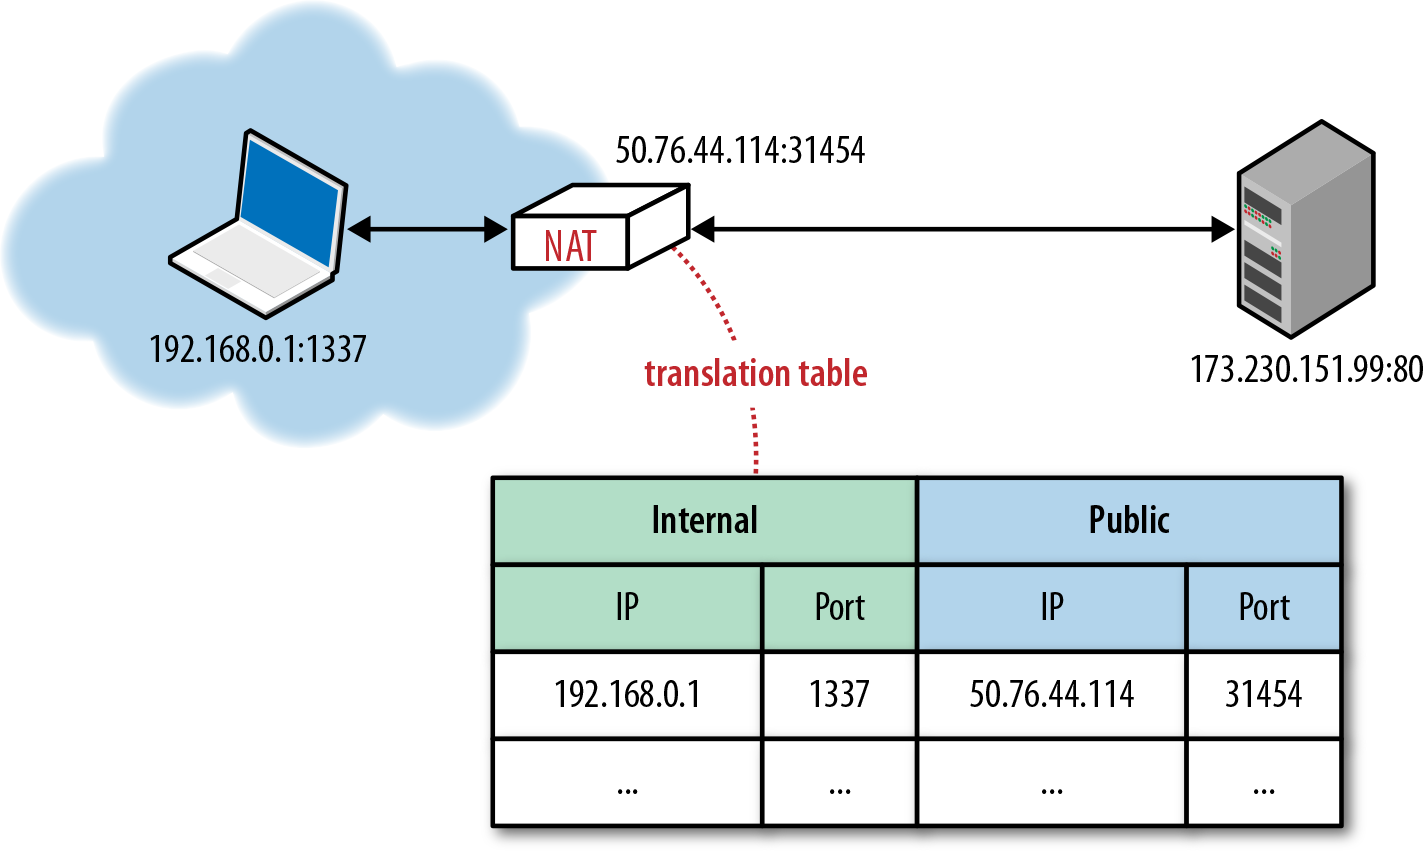
\includegraphics[width=\textwidth,height=0.2\paperheight,keepaspectratio
]{figures/nat}
\caption{A NAT maintains a table that maps an internal IP address and port to a public IP address and port.~\cite{NATIllustration:Online}.}
\label{fig:NAT}
\end{figure}

The presence of NATs can pose problems to applications leveraging the UDP protocol for transportation of data and network communication in general. The different techniques that can be used to resolve problems caused by NATs are often referred to as \emph{NAT Traversal} techniques.

The underlying issue with the UDP protocol is the absence of state, as opposed to the TCP protocol. The statelessness of the UDP protocol makes it difficult for a NAT to determine when a table entry is no longer relevant and should be dropped, which leads to the fact that UDP routing entries are expired based on time. If an entry is predeterminedly expired, it will cause inbound packets to be dropped since they cannot reach the source. In the case of TCP, which has a well defined state, it is inherently simple to determine when an entry should be dropped.

A technique commonly used to solve the problem with UDP entries expiring and being dropped is to utilize keepalives at regular intervals. This is commonly referred to as \emph{UDP hole punching}~\cite{UDPHolePunching:Online}.

Another problem is that internal hosts know their internal IP address but not their public one. If a host runs an application that communicates the IP address as a part of the payload to hosts outside of the private network, there would obviously be a mismatch if they communicate their internal address. It is therefore common to utilize a protocol called STUN (Session Traversal Utilities for NAT)~\cite{RFC5389:Online}. STUN enables hosts to obtain their public IP addresses with the help of an external STUN server (See figure~\ref{fig:WebRTC - STUN}).

\begin{figure}[htp]
\centering
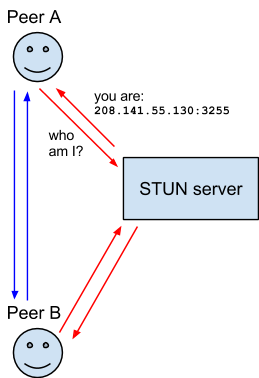
\includegraphics[width=\textwidth,height=0.2\paperheight,keepaspectratio
]{figures/webrtc-stun}
\caption{STUN servers let peers in a private network behind firewalls discover their public IP-addresses~\cite{WebRTCArchitecture:2014:Online}.}
\label{fig:WebRTC - STUN}
\end{figure}

The mentioned techniques are not always adequate because of the fact that STUN does not work with all types of NATs. In some cases, UDP traffic might be blocked by a firewall. To solve this issue, another protocol called TURN (Traversal Using Relays around NAT) protocol~\cite{RFC5766:Online} is used. TURN establishes a TCP connection with a relay server if UDP fails. The relay server is used to tunnel data to the other host, which means that there is no longer a direct peer-to-peer connection (See figure~\ref{fig:WebRTC - TURN}).

\begin{figure}[htp]
\centering
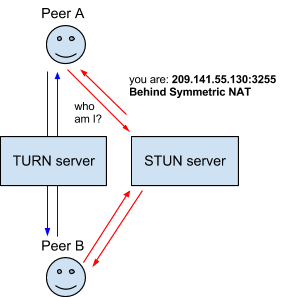
\includegraphics[width=\textwidth,height=0.2\paperheight,keepaspectratio
]{figures/webrtc-turn}
\caption{If a peer-to-peer connection cannot be established, a relay through a TURN server could be used. All peers send their packets through the relay which makes it more costly. But at least the connection works~\cite{WebRTCArchitecture:2014:Online}.}
\label{fig:WebRTC - TURN}
\end{figure}

\subsection{WebRTC}

Up until recently, browsers lacked support for direct peer-to-peer communication. In 2011, however, Google released a project called WebRTC, with the purpose to enabling real-time voice and video streams in the browser~\cite{WebRTCMemo:Online}. Since then, WebRTC has evolved to enable more general real-time data communication between browsers~\cite{WebRTC:Online}. The technology became usable for arbitrary data streams in major browsers in 2014~\cite{WebRTCChrome:Online}~\cite{WebRTCFirefox:Online}.

Since the announcement of WebRTC, the organizations W3C and IETF has been working together on standardizing protocols and drafting APIs. The major browser vendors Google, Mozilla, and Opera support the project~\cite{WebRTCAndMicrosoft:2012:Online}. While Microsoft supports the concept of WebRTC and contributes to the W3C WebRTC working group, the company does not support Google's (or nowadays, W3C's and IETF's) version of it~\cite{WebRTCAndMicrosoft:2012:Online}. Microsoft does not want to support the new technology until it has become a standard and does not fully agree on some constraints placed on it~\cite{WebRTCAndMicrosoft:2012:Online}. Microsoft states that one of their issues with the current WebRTC version is that it has predetermined paths for choosing codecs and ways of sending media over the network – sort of a black box. This hinders application developers who want to optimize to suit their own needs. Microsoft's answer to this is their own CU-RTC-WEB (Customizable, Ubiquitous Real Time Communication over the Web) which attempts to address these issues.

WebRTC's functionality is abstracted into three different APIs: \emph{MediaStream}, \emph{RTCPeerConnection} and \emph{RTCDataChannel}~\cite{WebRTCBasics:2012:Online}. MediaStream, or \emph{getUserMedia}, handles synchronized media streams, i.e. synchronized video and sound from a computer's camera and microphone. RTCPeerConnection manages reliable and efficient communication of arbitrary data streams, it utilizes techniques such as \emph{jitter buffering} and \emph{echo cancellation} to ensure a high standard even in unstable networks. For the intent of file sharing, the RTCDataChannel API is the most relevant.

% Introduce that WebRTC builds on top of UDP
At the transport layer, WebRTC makes use of UDP which can be motivated by the fact that timeliness is vital for real-time communication~\cite{HighPerfBrowserNetworking:Online}. The UDP protocol alone is not enough to construct efficient peer-to-peer applications. For this reason, WebRTC adds a number of additional protocols on top of UDP (See figure~\ref{fig:WebRTCProtocols}).

WebRTC's usage of UDP makes peer-to-peer communication inclined to suffer from connectivity problems in the presence of NATs. This problem has been taken into account and is relieved by utilizing the Interactive Connection Establishment (ICE) protocol~\cite{RFC5245:Online}. The ICE protocol handles NAT Traversal and is used for establishing peer-to-peer connections. It makes use of STUN and falls back to TURN when no other alternatives exists (See figure~\ref{fig:ICE}).

For the sake of security, data is encrypted according to the DTLS (Datagram Transport Layer Security) protocol. The DTLS protocol is based on the TLS (Transport Layer Security) protocol, the main difference being that DTLS is constructed for datagrams while TLS is used for reliable transport protocols such as TCP.
% udp does not guarantee that much, introduce some other protcols that helps

% insert protocol stack
\begin{figure}[htp]
\centering
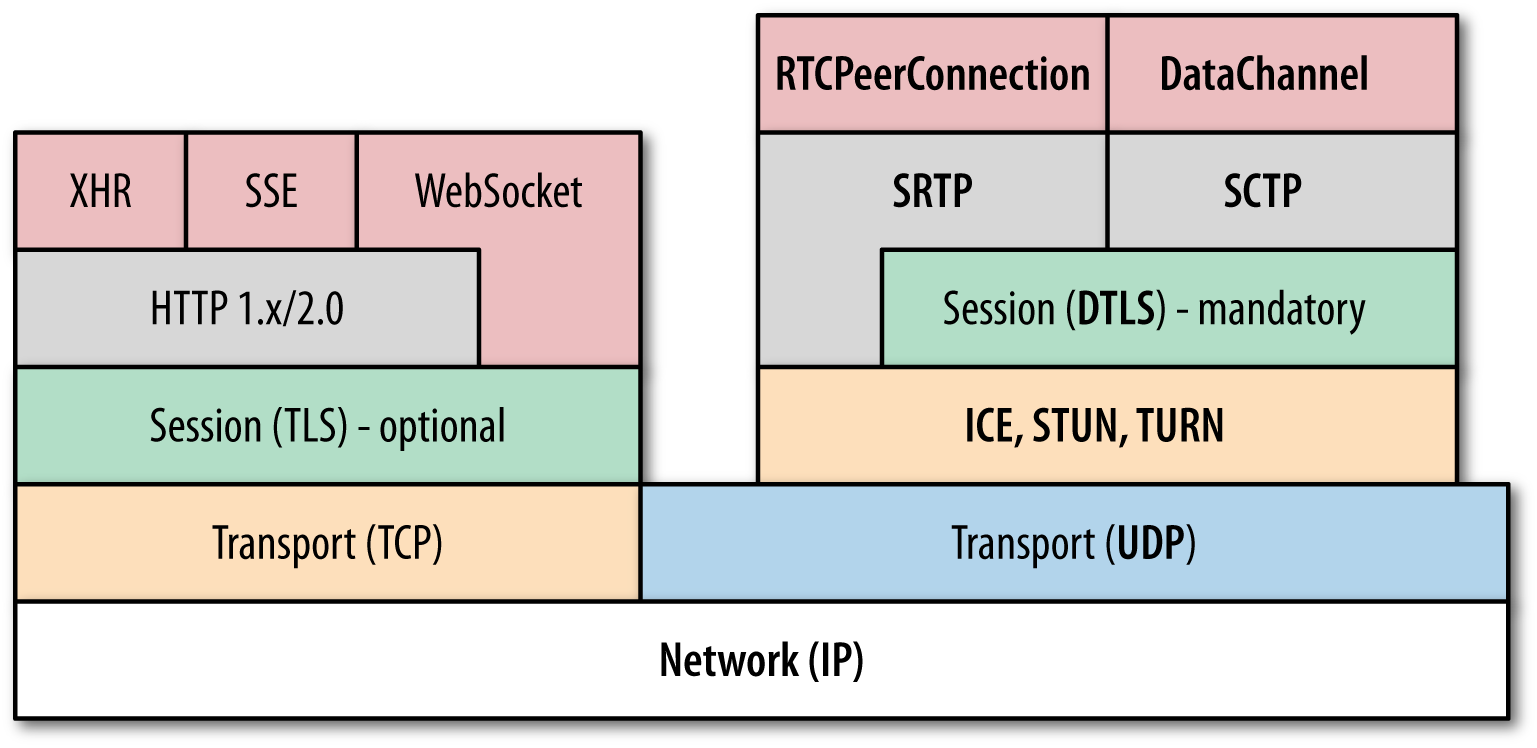
\includegraphics[width=\textwidth,height=0.25\paperheight,keepaspectratio
]{figures/webrtc_protocol_stack}
\caption{The underlying protocols of WebRTC~\cite{WebRTCProtocolStack:Online}}
\label{fig:WebRTCProtocols}
\end{figure}

% Data transfers are encrypted with the DTLS protcol

\subsubsection{RTCPeerConnection}
\label{subsubsec:rtcpeerconnection}
The RTCPeerConnection API handles the creation of peer-to-peer connections and takes care of connectivity problems caused by NATs (see section~\ref{subsec:nattraversal}) by utilizing the ICE protocol. 

\begin{figure}[htp]
\centering
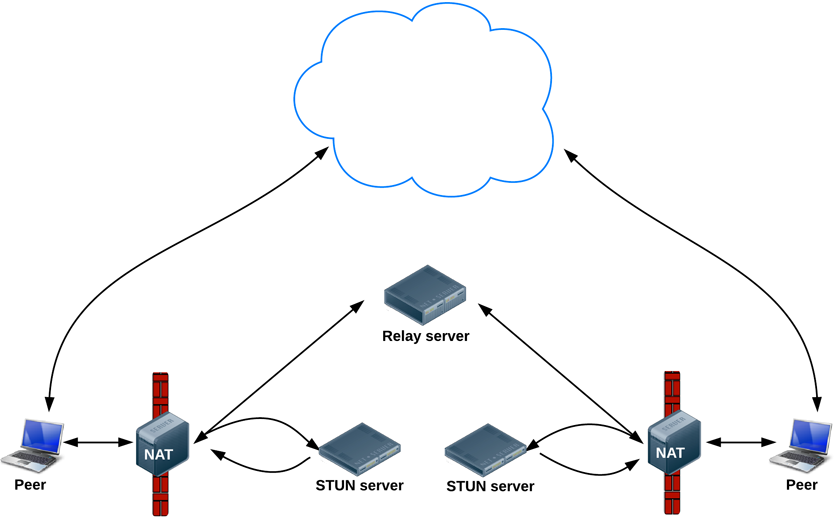
\includegraphics[width=\textwidth,height=0.25\paperheight,keepaspectratio
]{figures/ICE}
\caption{{The different ways for ICE to find network interfaces and ports, titled \emph{Finding connection candidates}~\cite{WebRTCBasics:2012:Online}, available under a Creative Commons Attribution 3.0 Unported License\protect\footnotemark}}
\label{fig:ICE}
\end{figure}

\footnotetext{http://creativecommons.org/licenses/by/3.0/legalcode} %Footnote text to ICE figure caption

Before a connection can be initiated between peers, one of two parts must extend an offer which contains data describing the connection to the other part - this is often referred to as the signaling phase. The signaling phase depends on two things:

\begin{itemize}
  \item The existence of a signaling channel - where a connection should be negotiated
  \item The choice of signaling protocol - which protocol that should be used for the negotiation
\end{itemize}

Regarding the choice of signaling channel, a dedicated signaling server is often used. That is, a server which relays connection offers from one peer to another. Although this is the most common choice of signaling channel, examples of a more serverless approach can be found~\cite{webrtcsignalserver}. The standard does not provide any recommendations regarding the choice of a signaling protocol - this is for developers to decide.

\subsubsection{RTCDataChannel}
The RTCDataChannel API allows for arbitrary data to be sent peer-to-peer by leveraging the RTCPeerConnection API. As UDP itself - which WebRTC runs on top of - is not suitable for reliable data transportation, the RTCDataChannel API utilizes the SCTP (Stream Control Transport Protocol) protocol. SCTP can be configured in terms of reliability and message order, and it provides some additional services such as congestion and flow control~\cite{HighPerfBrowserNetworking:Online}.

\section{Distributed storage}
\label{sec:distributedstorage}
With the inherent problems of trust in CAs in a PKI, several approaches to publicly available distribution of cryptographic keys have emerged in recent years. Some use a blockchain-based approach derived from Bitcoin. This implies distributing a cryptographically based ledger over an entire network and taking it beyond that of a monetary currency to systems that can be used for a wider range of applications. There are also other ideas on how to solve the trust issue.

\subsection{Namecoin}
A phenomenon that has been on the rise during recent years is that of cryptocurrencies such as Bitcoin~\cite{nakamoto:2009}. A cryptocurrency is a virtual currency that builds on cryptographical principles to ensure integrity and consistency. Each participant in the Bitcoin network keeps a ledger of all transactions throughout the history of the network. This ledger is called the \emph{blockchain}, because it is a chain of \emph{blocks}. Each block constitutes of the hash of the previously generated block, a number of other recent transactions and a salt. In order for a transaction to be deemed valid, it needs to be included in one of these blocks. This inclusion is done by volunteering nodes that perform a brute-force search for a salt that generates a block hash of a specific form. When such a salt has been found, the block is included in the blockchain. This search for salts is called \emph{mining} and constitutes the work done by \emph{miners} to keep the network running. As an incentive, each verified block also includes a reward to the miner that finds the salt. In effect, all transactions ever made are publicly available and tracked so that anyone can confirm their validity. This prevents forgery and double-spending of bitcoins.

Namecoin~\cite{Namecoin:Online}, another cryptocurrency, is essentially a fork of Bitcoin with new transaction types that allows its blockchain to be utilized as a distributed key-value store. Although similar in nature to Bitcoin, its main purpose is to be used as a decentralized domain name system (DNS), rather than as a monetary currency. With a decentralized DNS such as Namecoin, top level domains (such as \emph{.com} or \emph{.se}) can exist without being controlled by any central authority~\cite{Coindesk:2013:Online}. Also, the DNS lookup tables where domain names and their IP addresses are stored are shared in a peer-to-peer manner. The only necessary condition for these domains to be accessible is that there are participants willing to run the DNS server software. Although mainly intended to be used as a DNS, it contains several namespaces where arbitrary strings such as public cryptographic keys can be stored.

\subsection{Ethereum}
Bitcoin and its derivatives have a built-in scripting language that runs on top of the blockchain. It has limited functionality and is mainly used to set up contracts and multi-party-signed transactions that enables escrow-like functionality. Ethereum~\cite{Ethereum:Online} is a novel crypto-currency built from scratch that extends this idea by building on \emph{smart contracts} using a Turing complete domain specific language. This makes it a platform for building arbitrary distributed system. Users running code pay a small fee of the internal currency \emph{ether} for each computational step. Ethereum could therefore work not only as a DHT, but also execute parts of system logic. Development of Ethereum was announced at the end of 2013 and has a planned first release in late 2014.

\subsection{Keybase}
Keybase~\cite{Keybase:Online} is another recent initiative that intends to solve the distribution of public keys. It is essentially an HTTP-interface that maps keys to identities. While keys themselves are stored centrally at Keybase's servers, it utilizes social media for proofs. The idea is that a Keybase user will put proofs of their Keybase identity on public social media services such as Twitter or Github. The Keybase client will refer to these to make sure that the given key corresponds to the user of these social media accounts. It ties identities to keys as long as a user's Keybase and social media accounts are not all compromised.

\section{Cryptography}
\label{sec:techcryptography}
Encryption is the process of running data through an algorithm with the goal of making the information unreadable for unauthorized parties. The output of an algorithm depends on the input data and the \emph{encryption key} used. There are two types of key schemes: symmetric-key schemes and asymmetric-key schemes (also known as public-private). In symmetric cryptography  schemes such as AES, the same key is used for both encryption and decryption. Because of this, both sender and recipient must possess the same key, and the key must therefore somehow be communicated through a secure channel. Asymmetric key-schemes such as RSA, on the other hand, work with pairs of keys where the encryption of one corresponds to the decryption of the other. One of these keys is called \emph{private} and should only be known to the person generating the key-pair, and the other is called \emph{public} and can be shared freely. In this way, there is no problem with how to transmit keys. Generally, encryption and decryption in asymmetric schemes are much more computationally demanding than that of symmetric schemes, so a common approach is to use symmetric encryption for data and asymmetric keys for the communication of the symmetric key.

Until recently, the practice of performing cryptographic operations in a web browser environment has been considered bad practice by security professionals~\cite{Matasano:Online}. One reason for this is that it has been impossible to verify the integrity of client-side source code between executions - something that has now changed with the advent of signed browser extensions. Another issue is the internal openness of JavaScript - any cryptographic implementation would unavoidably expose all their primitives\footnote{The basic functions in a cryptographic scheme such as hashing, encryption, decryption, signing, verification and generation of keys}, as well as raw private and secret key data. With the advent of the new Web Cryptography API, or \emph{WebCrypto}, these issues are being addressed~\cite{WebCrypto:Online}.

\subsection{Web Cryptography API}
WebCrypto is an open standard for implementation of cryptographic primitives accessible through web client code~\cite{WebCrypto:Online}. Basically, all primitives and raw material (the underlying keys and algorithms) would be blackboxed for the client application and executed natively in the web browser. However, the API is still in an early stage and at the time of this writing only Chromium~\cite{ImplementedChromium:Online} and Microsoft Internet Explorer~\cite{WCAImplementationMicrosoft:Online}, out of the major browsers have implemented more than a basic pseudo-random number generator~\cite{WCAImplementationMozilla:Online}. The exact implementation of the different features may come to change drastically over time.

\subsection{Certificates}
% TODO: Explain usage of X.509 and why it's relevant
Certificates are used to confirm the validity of users' keys~\cite{EETimesCrypto:Online}. Instead of requesting keys directly, which could have potentially been compromised by malicious third parties, certificates are retrieved from trusted CAs. In essence, a certificate contains a user's public key along with user data and information about the certificate. The CA signs the certificate and a hash is embedded as proof that the certificate has not been unlawfully modified.

These certificates are structured according to a certain format. One commonly used format for certificates is the X.509 standard~\cite{IETFX509:Online}. In the X.509 system, a CA issues a certificate binding a public key to a name such as an e-mail address or a DNS entry.

\subsection{Advanced Encryption Standard}

% TODO: Explain relevance of algorithms in general as well as usage of AES and why it's relevant
The Advanced Encryption Standard~\cite{AES:2001}, \emph{AES}, is one of the most widespread symmetric encryption schemes in use today. It is a specification established by the U.S. National Institute of Standards and Technogy in 2001 and based on the Rijndael cipher~\cite{Rijndael:Online}, which in turn is based on the idea of substitution-permutation~\cite{AESISFAST:Online}. The algorithm distorts the inputed value by means of replacement and uses a structure with a fixed block size. AES was intended as a replacement for DES~\cite{DES:1977}~\cite{Cisco:2001}. Encryption is performed in rounds with the number of rounds depending on the length of the key.

For reasons of performance and security, symmetric algorithms such as AES encrypt data in blocks of fixed size. There are different ways to make these blocks relate to each other, depending on the type of data and application. One of the more common modes is Cipher Block Chaining, or CBC, where the encryption function for each subsequent block is fed the encrypted version of the previous block. This is done to make blocks with the same input plaintext indistinguishable~\cite{SearchSecurityCipherBlockChaining:Online}.
% Diffusion and confusions together will complicate statistics attacks and hides local patterns in the language.

\clearpage

\chapter{Related work}\label{chap:similar}
  There is a plethora of technologies for distributing and synchronizing data between peers that at a first glance may look very similar to Rymd. Below are some more well-known and similar pieces of software. The features described will hopefully highlight how they relate to each other and Rymd.

\begin{description}
  \item[Bittorrent Sync] \cite{BitTorent:2014:Online} is a distributed peer-to-peer multi-way file syncing software using the Bittorrent protocol for file transfers. Synchronized folders are mapped directly to the underlying file system, and each folder is encrypted using a shared secret key. Public-key cryptography is not employed, and the only available clients are closed-source binary applications using the network of the creator, Bittorrent Inc. While they do have a developer API, it requires developer keys issued from Bittorrent Inc.
  \item[RetroShare] \cite{Retroshare:2014:Online} markets itself as a Friend-2-Friend decentralized communication platform which uses GPG to create a Web of Trust between peers. It is, however, a very large project: The application provides file-sharing, instant messaging, discussion forums, e-mail, Voice over IP (VoIP) and group chat. It is open source and distributed as cross-platform binaries.
  \item[ShareFest] \cite{Sharefest:2014:Online} is a peer-to-peer one-to-many file-sharing web based software using WebRTC data channels. ShareFest can be seen as a more limited and primitive version of what Rymd aims to be: ShareFest can share files over WebRTC channels, but does not accommodate authentication, persistence or local encryption. It does, however, operate on a mesh network similar to Bittorrent. Other similar WebRTC-based P2P file sharing web applications but without additional cryptographic properties include RTCCopy and ShareDrop.
  \item[Freenet] \cite{Freenet:2014:Online} is one of the first \emph{darknets}, consisting of a distributed, decentralized data store that uploads files with strong anonymity across a network. Each node in the network also acts as a cache for the content stored in the network. Files are generally split up in parts that are distributed, and when fetching files it is unfeasible to determine the origin and sender of the files. Focusing on anonymity, free speech and plausible deniability, the encryption is done in the communication and storage layers. Because of this design, Freenet is quite slow. Files can be retrieved using the cryptographic key used to upload them. Freenet is free software built with Java.
  \item[Tahoe-LAFS] \cite{Tahoe:2014:Online}, or Tahoe Least-Authority Filesystem, is a distributed, encrypted and redundant file system. It distributes encrypted files across a predetermined set of servers and allows sharing of both mutable and immutable files. There is a web-interface, but like all other user-interfaces it has to go through a \emph{gateway} where encryption and server-communication is performed. Users will typically run their own gateways and will thus need to accommodate hosting for them.
  \item[Bitmessage] \cite{Bitmessage:2014:Online} is a P2P distributed messaging system intended to replace e-mail. Public keys of all participants are distributed over the entire network, and can be retrieved using their fingerprints (which are used as addresses). In order to send a message, it is encrypted using the receiver's public key and sent to the entire network. Participants try to decrypt every message, and will so be able to retrieve the ones they can decrypt. Messages are stored in the network for two days. There is thus no way to tie messages to senders and recipients.

\end{description}

Rymd differentiates by being the only project so far that combines the properties of open source, purely web based, decentralized and cryptographically secured. Additionally, it is a developer-geared library rather than a user-oriented application.

\clearpage

\chapter{Analysis and System design}\label{chap:design}
  \section{Peer-to-Peer Communication}

\section{Identities, DHT and the Blockchain}

\section{Decentralization}

% "Centralized control – Distributed Data Architectures"
% http://highscalability.com/blog/2014/4/7/google-finds-centralized-control-distributed-data-architectu.html
% / Johan

\section{Encryption}

\section{Data Storage}

\section{Modularity}

\clearpage

\chapter{System implementation}\label{chap:implementation}
  % TODO This chapter *must* detail our implementation of the modules introduced in System Design!

With the background of the high-level foundations presented in chapter\ref{chap:design}, this chapter details the underlying implementation of the modules of the whole system. All source code has been written in JavaScript. \texttt{DHT} is run as a Node.js server and \texttt{Shuttle} runs as a web application. Rymd is the platform independent core module containing the business logic of the system. All other modules contain the specific implementations for each problem area.

\section{Rymd}
\label{sec:rymd}

% TODO Somebody

The source code is available at: https://github.com/rymdjs/rymd. The Rymd library is the only truly implementation-agnostic module and should be runnable on any platform as long as implementation modules are dependency injected. 

\section{Shuttle}
\label{sec:shuttle}
The front-end prototype was built in order to test and implement the features of Rymd. Early versions included a minimum viable interface for adding, showing and sending files. This was further iterated over, ending up letting the user:

\begin{itemize}
  \item Add files through form control or drag-and-drop
  \item Share, view and delete files
  \item Login (verifies with the DHT, see~\ref{sec:authentication})
  \item Get in-app notifications for incoming sharing requests
  \item Download remote files that have been shared by other users
  \item Add custom encryption keys
\end{itemize}

The source code is available at: https://github.com/rymdjs/prototype.

Shuttle uses Rymd's functionality by instantiating a global \texttt{RymdNode} object (see~\ref{sec:rymd}). This effectively makes Shuttle a node in the network. In-app notifications are shown by listening to certain events on the \texttt{rymdNode} object.

When the front-end Javascript code was beginning to grow fairly complex, a decision was made to rewrite the code for the front-end framework Backbone\footnote{http://backbonejs.org}. Backbone provides a barebones concept of models, collections, views and events, as well as a URL router. The prototype was thus restructured and integrated with Backbone's patterns.

\subsection{Persisting front-end models}

A major feature of Backbone is the ability to connect to an existing data API for persisting front-end models to a backend. By the use of \texttt{XMLHttpRequest} for asynchronous HTTP requests, Backbone is able to talk to a RESTful API when creating, reading, updating or deleting models. However, in Shuttle the data should not be persisted to a remote server, but instead use the local data store in Rymd (see~\ref{sec:indexeddbstore}). A custom adapter was written\footnote{https://github.com/rymdjs/prototype/blob/develop/lib/Backbone.ResourceStore.js}, which intercepts Backbone's calls by overriding the \texttt{sync} method to make it communicate with the local store with CRUD actions.

\begin{Code}
\begin{lstlisting}[caption={Sample scenario of persisting models}, label={lst:backbonesync}]

// The custom overriden adapter for persisting to a local store
var ResourceStore = require("../Backbone.ResourceStore");

// Define a new collection using the adapter above
var ResourcesCollection = Backbone.Collection.extend({
  model: File,

  initialize: function() {
    // Inject App.rymdNode.store, which is an instance of the IndexedDBStore module
    this.resourceStore = new ResourceStore(App.rymdNode.store);
  }
});

// Backbone Collection for in-memory storage of models
var myFiles = new ResourcesCollection();

// Populate the collection with file models from the local store
myFiles.fetch();

// Create a file model for the collection. The model is now automatically saved to the local store,
// thanks to the above mentioned adapter.
myFiles.create(new File());
\end{lstlisting}
\end{Code}

\section{Authentication (DHT, DHT Client)}
\label{sec:authentication}
Since the default authentication implementation utilizes Namecoin, which can not be accessed directly from a web application, a gateway service needs to be used. Therefore, the domain of authentication spans over several parts in separate systems:

\begin{description}
  \item[DHT] A NodeJS\footnote{http://nodejs.org} based server that looks up entries in the Namecoin blockchain. It is also used to keep track of session-based IDs, as described under~\ref{sec:communication}. This is the only module that runs outside of the Rymd library.
  \item[DHT-Client] Client-side interface module to the DHT.
  \item[ConnectionHandler] Submodule in the Rymd library. Implements the Needham-Schroeder-Lowe authentication business logic.
\end{description}

The idea with this separation is that the authentication algorithm is part of the core library, while derivative projects should be able to replace $DHT$ and $DHT-client$ with implementations using other stores like Ethereum or Keybase without having to consider writing a secure authentication protocol, should they so desire.

The source code is available at: https://github.com/rymdjs/dht-client and https://github.com/rymdjs/dht.

\section{RymdCrypto}
\label{sec:cryptography}
%TODO: Rewrite, explain "secure primitives". Probably this whole sentence should be removed./Robert
%In Rymd, security is achieved through secure primitives, user restrictions and by the use of cryptographic communication libraries.
% uses the Web Crypto Api for encryption (3AES - 1024) ,decryption key import and export ,
At this stage Rymd only runs in the very recent development versions of Google Chrome or Chromium. The implementations provided by these browsers supply key generation but there is no support for persisting keys between sessions or even exporting private keys. W3C - the organization behind the WebCrypto API - have announced their intention to handle persistent key storage in an upcoming API called WebCrypto Key Discovery \cite{WebCryptoKeyDiscovery:Online}. However, Google has no intention of implementing this before the WebCrypto API is finalized. WebCrypto Key Discovery API was originally intended to be a part of the WebCrypto API but was extracted in favor of decreased implementation complexity. Before the WebCrypto Key Discovery API is implemented, the RymdCrypto module generates keys on its own. Doing this is bad practice and is only performed in order to get a prototype running.

The source code is available at: https://github.com/rymdjs/crypto.

\subsection{Dependencies}
The Crypto module is based around the use of cryptographic communication libraries; the module is strutured in a way such that cryptoback.js handles key generation and parsing while the rest is handled by the crypto.js module.
\begin{Code}
\begin{lstlisting}[caption={Included database operations}, label={lst:api}]
 //dependecies cryptoback.js
  var rsa = require('bignumber-jt'),
      Q = require('q');

 //dependecies crypto.js
  var root = this,
    Q = require('q'),
    cryptojs = require('crypto-js'),
    utils = require("./cryptoback");
\end{lstlisting}
\end{Code}
As previously mentioned, the Web Crypto API lacks functionality for storing keys between sessions or even exporting private keys. In order to support key storage between sessions, the key generation is moved out of the API and handled by a library \emph{bignumber-jt} \cite{Bignumber:Online}; The key is then parsed to a certificate.
All certificate have a static key size where asymmetric keys are of $1024bits$ and symmetric ($AES-CBC$) are of $256bits$; none are explicitly generated via the API.

%\subsection{Interface}
% before it's imported into its low-level interface. %TODO: Proper reference
%\begin{Code}
%\begin{lstlisting}[caption={Common database operations}, label={lst:api}]
% generateKeyPair: function() -> Promise({Uint8array,Uint8array})
% exportKey: function(WebCrypto::Key) -> Promise({Uint8array})
% importKey: function(String,Uint8array) -> Promise(WebCrypto::Key)
% signKey: function(WebCrypto::Key,Uint8Array) -> Promise
% verifyKey: function(WebCrypto::Key,Uint8Array,Uint8Array) -> Promise
% encrypt**: function(WebCrypto::Key,Uint8Array??) -> Promise(Arraybuffer)
% decrypt**: function(WebCrypto::Key,Uint8Array??) -> Promise(Arraybuffer)
% hash**: function(blob)  -> Promise(blob)
% generateSymmetricKey: function() -> Promise(WebCrypto::Key)
% \end{lstlisting}
%\end{Code}

% TODO Robert/Robin: Oversee this.
\subsection{Algorithms}
The Encryption uses two algorithms, namely the $RSAES-PKCS1-v1.5$ and the $AES-CBC$.
AES-CBC is a symmetric key AES based using cipher block chaining; it is the only symmetric algorithm implemented at the time of writing, besides it is fast\cite{AESISFAST:Online} and simple to use.
$RSAES-PKCS1-v1.5$ - an AES implementation based on the RSA algorithm.
The signing uses $RSASSA-PKCS1-v1_5$. This choice is motivated by the lack of alternatives and the fact the the Web Crypto API recommends the use of this algorithm on their web page. Finally, there are no other RSA signing algorithms included in the Web Crypto API.
A motivation for the use of SHA-256 could be found in the Decentralization section.
\begin{Code}
\begin{lstlisting}[caption={Algorithms implemented}, label={lst:api}]
  var generationAlgorithmSign =  {
    name: "RSASSA-PKCS1-v1_5",
    modulusLength: 2048,
    publicExponent: new Uint8Array([0x01, 0x00, 0x01]),
    hash: {
      name: "SHA-256"
    }
  },

  generationAlgorithmEncrypt =  {
    name: "RSAES-PKCS1-v1_5",
    modulusLength: 2048,
    publicExponent: new Uint8Array([0x01, 0x00, 0x01])
  },

  aesAlgorithmKeyGen = {
    name: "AES-CBC",
    length: 256
  },

 specFormats ={
    public: 'spki',
    private: 'pkcs8',
    secret: 'raw'
  }
\end{lstlisting}
\end{Code}
Regarding $RSAES-PKCS1-v1.5$, the fact that it uses RSA is inline with our guidelines since it allows the key to be reused for both signing and encryption (se table \ref{table:webcrypoapi})..
Considering DSA algorithms: the DSA is faster for signing and key generating but slower when it comes to signature checking and it also lack the ability to preform encryption.
Regarding accessibility, both algorithms are included in the Web Crypto API and are therefore provided by the browser as black boxes.
% add text about hashing
% why is the hashing in
\begin{table}[h]
\centering
\begin{tabular}{lcccccc}
Algorithm name & Type & Encrypt & Decrypt & Sign & Verify & ImportKey \\
RSAES-PKCS1-v1\_5 & ASYM & x & x &  &  & x \\
RSASSA-PKCS1-v1\_5 & ASYM &  &  & x & x & x \\
RSA-PSS & ASYM &  &  & x & x & x \\
RSA-OAEP & ASYM & x & x &  &  & x \\
ECDSA & ASYM &  &  & x & x & x \\
AES-CTR & SYM & x & x &  &  & x \\
AES-CBC & SYM & x & x &  &  & x \\
AES-CMAC & SYM &  &  & x & x & x \\
AES-GCM & SYM & x & x &  &  & x \\
AES-CFB & SYM & x & x &  &  & x
\end{tabular}
\caption{Some Web Cryptp Api Algorithms}
\label{table:webcrypoapi}
\end{table}
In commercial terms as for our project, RSA is clearly the winner; commercial RSA certificates are much more widely deployed than DSA certificates.
Furthermore, the asymmetric keys are wrapped in PKCS\#8 and SPKI certificates while the symmetric key exist in raw format.
The Private-Key Information Syntax Standard (PKCS\#8) -  defines a way to store the private key and the Simple public key infrastructure (SPKI) - defines a way to store the public key.
All three standards was chosen because they are the only three formats that is currently supported by Chromium \cite{ImplementedChromium:Online}.

% TODO Johannes

\section{IndexedDBStore}
\label{sec:indexeddbstore}

The main task for the data storage module was to abstract away the low-level methods in IndexedDB (the backing store used, see section~\ref{sec:indexeddb}). An API example can be found in listing~\ref{lst:api}. The module supports use of multiple object stores and auto-generation of GUID keys.

The source code is available at: https://github.com/rymdjs/data-storage.

\begin{Code}
\begin{lstlisting}[caption={Common database operations}, label={lst:api}]
var IndexedDbStore = require("indexeddbstore")

var Store = new IndexedDbStore("myStore")

// Fetch all records as an array
Store.all().then(function(records) { ... })

// Create a record
Store.create("A record").then(function(record){ ... })

// Insert a record
Store.save("A record").then(function(guid){ ... })

// Fetch a record by GUID
Store.get(guid).then(function(record) { ... })

// Delete a record by GUID
Store.destroy(guid).then(function(record) { ... })
\end{lstlisting}
\end{Code}

The largest challenge came to the edge cases when storing files, or as they are called in web browser: \emph{Blobs}. Since at present only Firefox can store blobs directly in IndexedDB, an alternate route had to be taken for other browsers. Initially the module used conditionals and converted incoming data to and from \emph{ArrayBuffers} (the browser construct for raw byte streams). But since ArrayBuffers are just the raw data, all metadata for the blobs (such as filename, timestamps, size) would be lost when saving as an ArrayBuffer. In early versions of the data storage module this metadata would be stored in a separate store in the database, but this was too tightly coupled and was removed. The final implementation is storing data as-is – any metadata must be saved explicitly in a separate operation.

The asynchronous API of IndexedDB is relatively verbose and complex. It makes heavy use of event driven programming and thus the developer communicates with the database with callbacks. By the use of \emph{Promises}\footnote{http://en.wikipedia.org/wiki/Promise\_(programming)}, the asynchronous, callback-based methods in the IndexedDB API was made streamlined and simple to manage.

\section{PeerJS Connection}
\label{sec:p2p}

% TODO: Niklas

% - built on top of peerjs, TODO (not sure how to reference to github)
Rymd leverages the open source project PeerJS\footnote{http://peerjs.com}, which simplifies sending peer-to-peer data between clients. PeerJS utilizes WebRTC and is essentially split into two components: a server which acts as the signaling channel, and a client side API which interacts with the server as well as other peers. The server only handles the brokering of connections, which implies that only the data necessary for negotiating a connection is sent through this point. For communication between the server and the clients, that is the signaling protocol, PeerJS utilizes both WebSockets and XMLHttpRequest \cite{PeerjsGithub:2014:Online}. After a connection has been setup between two clients, the server is no longer needed in order for them to communicate.

The source code is available at: https://github.com/rymdjs/peerjs-connection.

% - explain how peer.js works.
The following steps explain how PeerJS brokers connections:
\begin{enumerate}
\item Two clients connect to the PeerJS server, using the client side API.
\item The server returns unique IDs for each of the clients.
\item One of the clients connects to the other using the client side API, where the unique ID for the other one is provided. The PeerJS server then forwards the information needed to set up a peer-to-peer connection to the other client.
\end{enumerate}

In order to map the identity registered in the Namecoin blockchain to the ID supplied by the PeerJS server, the DHT service is used. After a client has connected to a PeerJS server, it supplies the data regarding the server IP and the generated ID to the DHT. When another client wants to create a peer-to-peer connection, it queries the DHT service for the Namecoin identity, which then returns the IP for the PeerJS server and the id for the client.

% write about identities and how these things are done

% short section about how fetching names from the dht service will needs to be protected

% modularity and such
In line with the project guidelines regarding modularity, PeerJS-specific code is separated into a module of its own. If the requirements are to change, then those changes are contained in a single module.

\section{Testing}
\label{sec:testing}

Automatic unit tests have been implemented where possible. Thanks to the use of isolated modules test suites were able to be short and concise. Mocha was used as test runner, with Chai as assertion library (please see section~\ref{sec:libraries} for links to external libraries used).

\begin{Code}
\begin{lstlisting}[caption={Sample test suite}, label={lst:testsuite}]
describe("IndexedDBStore", function() {

  var db;

  beforeEach(function() {
		db = new IndexedDBStore({
			dbName: "test"
		});
	});

  it("should have a database name", function() {
		db.name.should.equal("test");
	});

  it("should save a record and return an id", function() {
		return db.save({foo: "bar"})
		.then(function(id) {
			id.should.be.a("String");
		});
	});

  it("should retrieve a given record", function() {
		return db.save({foo: "bar"})
      .then(db.get.bind(db))
      .then(function(record) {

			record.should.be.an("Object");
			record.data.foo.should.equal("bar");
		});
	});
});
\end{lstlisting}
\end{Code}

No integration or functional tests have been written for testing larger parts of the system. This is due to the fast iteration of the library's interface and constant change in implementation.

\clearpage

\chapter{Results and Discussion}\label{chap:discussion}
  % TODO:
%   - Self-critical somewhere
%   - Ethical insights
Here, we go through the main goals with Rymd and see how well they could be met, where and why there are shortcomings and how these could be addressed. Finally, we explore the ethical motivation behind Rymd and the implications it could have in a non-technological sense.

\section{Could a truly decentralized system be achieved?}
One of the main initial goals with Rymd was to make the system truly decentralized and reliable independently of the availability of certain services. To a large extent, Rymd is successful in this area. Any application, including the prototype Shuttle, can be downloaded and executed locally. Therefore there are no dependencies on web servers, since all data transfers between clients are performed in a peer-to-peer fashion. No central database outside of the local client stores persistent data. There is, however, two parts where communication with central endpoints still needs to be done:

\subsection{WebRTC ICE}
As described in section~\ref{sec:p2p}, establishing of WebRTC connections still relies on the availability of a STUN or TURN server. This makes implementing applications depend on the availability of such a server. However, there are several public ICE servers available and in the case of downtime it is trivial to set up a new one and make the application use the new server instead. Also, since verification of identities of peers is performed locally and all data is end-to-end encrypted, there is no possibility of the administrator of these servers to spoof identities or deduce anything about shared resources. The two things that do leak are identity names (since these are needed to deduce who to connect to whom) and, if TURN is used, estimated size of data transferred. We found no way around the former and decided the latter to be a fair tradeoff - future implementations that care about leaking of resource size could solve this by also transfer redundant padding data regardless of resource size.

\subsection{Accessing the DHT}
The Namecoin blockchain is used to tie identities to their public keys and PeerJS endpoints. Since Namecoin (or any other currently existing cryptocurrency for that matter) communicates using their own binary data protocol\cite{BitcoinSource:2014:Online}, Rymd can not interact directly with the blockchain to fetch this information before a mutual peer-to-peer authenticated connectin is established. Therefore, an HTTP gateway running the Namecoin software was developed that acts as a bridge between the blockchain and Rymd nodes. Trust in the operator of this gateway is crucial, since public keys are fetched and verified through it. The paranoid user could, however, easily run their own gateway or manually verify or insert public keys using their own Namecoin client. On May 6th, at the time of writing of this report, a public and more general HTTP/Blockchain interface at \emph{chain-api.com}\cite{Chain:2014:Online} was released. Currently it only support Bitcoin, but promises future integration with the Namecoin blockchain. Once that happens, it would be trivial to replace the current gateway with Chain if one would like to do so. The buzz around services like these shows that this is an emerging area with more interesting development to come in the near future.

Something that would both solve these issues and be very interesting in many other areas is a blockchain where nodes can communicate through open web protocols. This would mean that web clients could interact directly with the blockchain without going through external gateways like these, at the same time allowing them to contribute to the network. Given the premises stated in the introduction and the rapid development of emerging blockchains and cryptocurrencies, we think it is only a matter of time before this happens.

\section{Is all data truly cryptographically secured?}
%TODO: Reference
In the application layer, all communication over WebRTC is DTLS encrypted. As stated in section XX, for local storage and sending of resources, every resource is also AES encrypted with a resource-specific key. Since all existing browser implementations of the Web Cryptography API are still experimental and partial and there is not yet support for secure storage of cryptographic keys, the keys are stored alongside their encrypted data in IndexedDB. As long as the keys are not passphrase protected, this effectively means that at the level of the local client, the encryption adds no extra protection and can be considered redundant. An adversary gaining access to the database with the encrypted data would also have access to the decryption key. This is most likely only during a transitional period and as the Web Crypto API becomes stable and fully implemented across browsers, separate key storage options will become available and this can be resolved.

Despite this problem, the AES encryption still serves a purpose. Consider an application utilizing Rymd where users communicate through each other in a \emph{darknet} fashion. In these cases it is imperative that resources can be transmitted separately from their keys and metadata so that intermediate peers can facilitate the transfer of resource data without gaining knowledge of the contents.

Also, systems with updateable resources can and should regenerate keys for each version and backward secrecy - the property that access to the key for one version of the resource will not allow decryption of older versions of that resource - will be achieved.

\section{Is the system modular and implementation agnostic?}
As much as Rymd uses and relies some of the latest web technologies, great care was taken during development to not make it rely on any of these implementations, should they be superceded or complemented by other, more fitting alternativces. The main Rymd library itself handles only the business logic of the system and gets the modules implementing data storage, cryptography, peer-to-peer communication and DHT interaction supplied at runtime via dependency injection. Developers who have their own idea of how these needs should be served in their projects could write their own implementation modules. The one area where work needs to be done is that currently, storage of keys, metadata and resource data are tied together. Before Rymd can go stable, this should be addressed by treating these as separate data stores alltogether even if the current implementation puts all three side by side in IndexedDB.

\section{Ethical aspects}
Rymd was originally conceived from an ethical issue: The one that free, private and secret communication should be easily accessible and usable on the web. As it currently stands, truly secret and private communication requires running binary files and/or putting trust in a service provider. Rymd aims to be a step away from that restriction.

\subsection{Does Rymd meet this goal?}
At its current state, Rymd should not be trusted with confidential data. This is mainly because of the limitations stated in the preceding sections that come from the choice of still immature, cutting-edge technnologies. Also, Rymd is still in an experimental stage and should not be considered stable or trusted until it has been exposed to extensive peer review and scrutiny by the community - a reservation that should be held for any project of this nature. However, we are confident that we are going in the right direction and hope that further development could make Rymd to a contributor in the movement of free communication on the web.

\subsection{Implications}
As always when it comes to services enabling private communication, concerns are raised on the issue of what they can be used for. Commonly mentioned are terrorism, drug dealing and child pornography. First, we want to emphasize that Rymd does not in itself provide any anonymity for its users (though it could easily be used in conjunction with anonymization services such as TOR\footnote{https://www.torproject.org}). While Rymd could indeed be used for these purposes, there are already other services such as the ones mentioned in~\ref{sec:similar} that are currenly used for these purposes - Rymd does not enable risks that are not already present.

Inevitably, the question of which party holds responsibility for villainy is raised when a project of this nature is realized. One could argue that we are the ones responsible since we are supplying end users with the possibility to perform malicious actions. Another claim could be that the government is the one to blame for allowing such services to exist. Our own opinion on this matter is that people are solely responsible for their own actions. Technology exploring new frontiers is always met with critical glaze; laws and regulations have merely briefly halted advancement. One way or another, technological evolution always prevails. Meanwhile, people performing atrocities will probably always find other ways of doing their deeds. It therefore seems resonable to try to stop people performing atrocities than the tecnology currently under the microscope.

Mainly, however, it is our opinion that the right to private and secure communication without corporation or government surveillance is a human right, and this right is effectively nonexistant if it requires significant monetary resources and/or technical know-how. Putting this standpoint aside, we have mainly treated this issue as a technical one and will let the reader of this report decide for themselves where they stand and how Rymd relates to this.

\clearpage

\chapter{Conclusion}\label{chap:conclusion}
  The scope of functionality that is included in open web standards is constantly widening, and with this so do the potentials and capabilities of modern web browsers. Some standards are still in their infancy. Most notably, the Web Crypto API is still in a experimental state and lack vital parts such as secure key storage. More progress is needed before secure authenticated peer-to-peer file sharing can be done by web browsers.

Even so, Rymd and Shuttle show that this future might not be that far away. Even if the resulting code is not yet ready for production from a security perspective, we feel that our ambition to create a starting point for a web-centered secure file sharing platform has gone well. It is our hope that Rymd will get feedback from the community in order to inspire and play a part in a new wave of file sharing technologies on the web.


\emph{``This is not the end. It's not even the beginning of the end. But it might be the end of the beginning.'' - Winston Churchill}

What this war is about is yet to be seen.

\clearpage

\nocite{*} % Cites everything from the bibliograph
\printbibliography% This command is new in biblatex. Do not attempt to use style files as with old latex.
\clearpage

% Appendices
\begin{appendices}
\pagenumbering{Roman}
\chapter{Communication flow}
  \subfile{appendices/flow.tex}
\clearpage
\chapter{List of external libraries}
  \label{sec:libraries}
  \subfile{appendices/libraries.tex}
\end{appendices}

\end{document}
